\chapter{Udledninger}  \label{bilag- statik udledning}

\section{Udledning af bøjningsspænding}  \label{bilag - Bøjningsspænding}

Spændingerne i stellet må ikke overstige materialets flydespænding. For at sikre, at dette ikke sker, laves der overslagsberegninger på spændingerne i de lineære bevægelser, der bruges til dimensionering af det endelige produkt. En skitse af udseendet af de lineære bevægelser fremgår af figur \ref{Skite af akser}.

\begin{figure}[H]
    \centering
    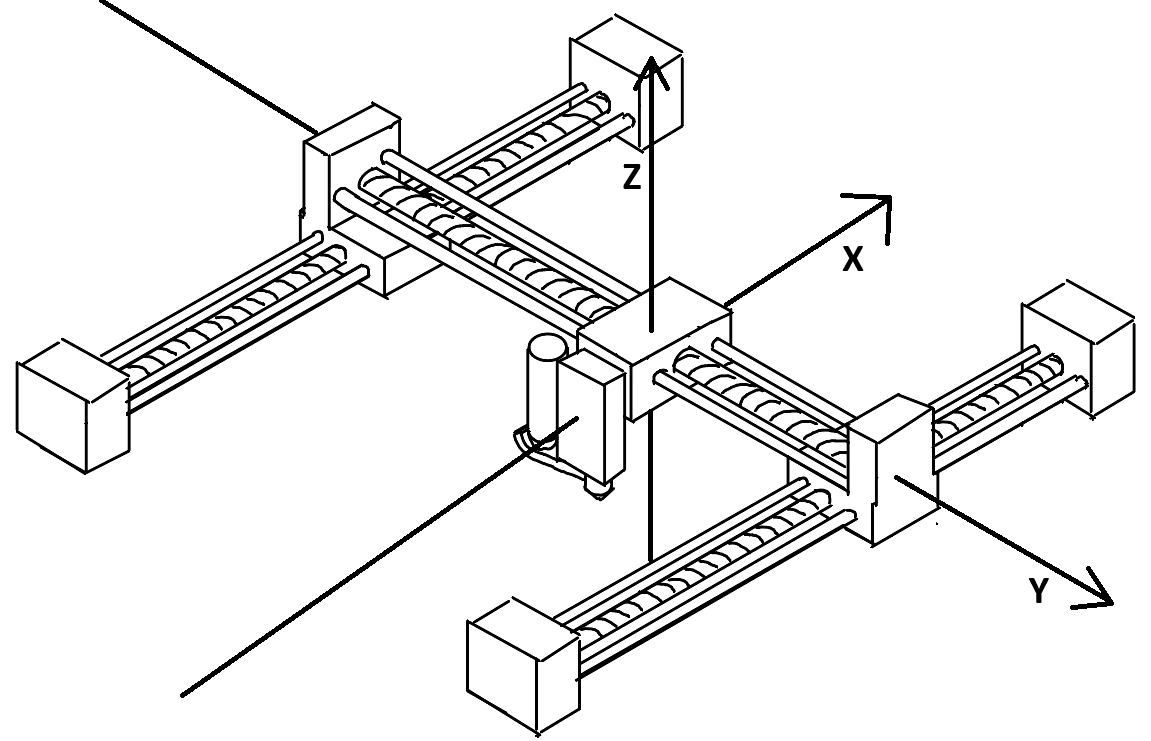
\includegraphics[width=0.6\linewidth]{Sections/6 Detaljeløsning/Media/Skitse af akser.png}
    \caption{Skite af akser}
    \label{Skite af akser}
\end{figure}

For at finde spændingerne, skal der defineres hvor og i hvilke retninger det er relevant at kigge på spændingerne. Hovedspændinger kan findes på to måder, gennem bøjning og gennem træk/tryk. I stængerne vil der være spændinger langs, og på tværs af akserne grundet accelerationer i disse retninger, samt bøjninger omkring hhv. xz-planet og yz-planet. Her vurderes det, at de største spændinger kommer i den retning hvor bøjning- og accelerationsspændinger vil kunne lægges sammen. Dette er for y-aksen i y-retningen og for x-aksen i x-retningen. For at finde de spændinger og derigennem undersøge de krav der stilles til stængernes tykkelse, vil de to spændingsformler udledes. 

For at undersøge spændingerne skal reaktionskræfterne findes. Her er det nødvendigt at udlede en formel for momentet igennem stængerne, samt normalkraftens størrelse i stangen, for at udlede formlen for spændingerne i stængerne. I dette afsnit vil der udledes en formel for normalspændingerne i y-aksen. Ligningenrne vil genbruges til x-aksen, da stængerne i x-aksen og y-aksen er stillet op på lige vis med samme randbetingelser og bevægelser, her varieres der kun i kræfterne.\\
Normalspændingerne i stængerne er todelte, de kommer fra træk og tryk, samt bøjning. Sammenhængen kan ses i formel \ref{formel: momentspænding} samt formel \ref{formel: Kraft over areal}.
\begin{equation} \label{formel: momentspænding}
    \sigma_{M(y)} = -\frac{M(y)}{I}\cdot z
\end{equation}
\begin{equation}\label{formel: Kraft over areal}
    \sigma_T=\frac{N}{A}
\end{equation}
Frit legeme diagram (FLD) for y-aksen ses i figur \ref{fig: FLD y}.
\begin{figure}[H]
    \centering
    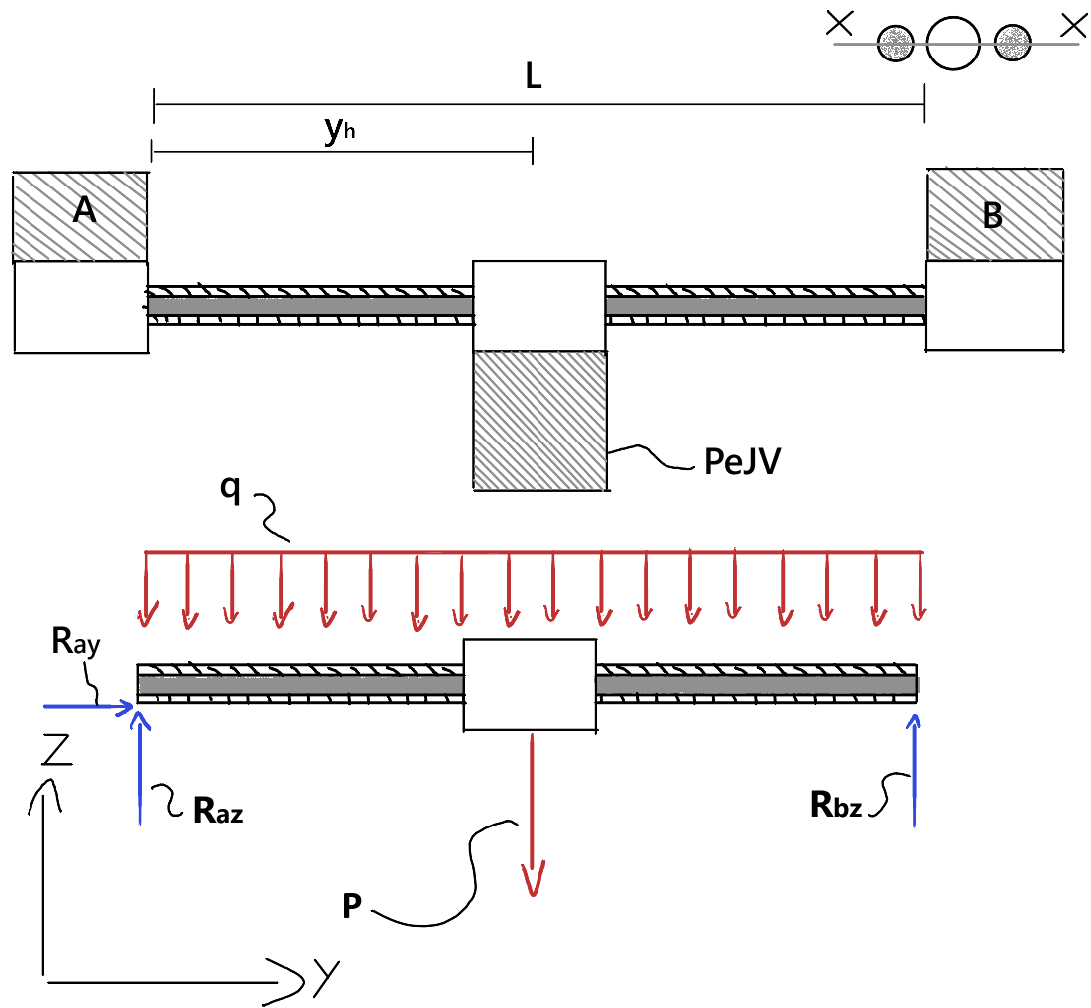
\includegraphics[width=0.6\linewidth]{Sections/6 Detaljeløsning/Media/FLD - y-akse.png}
    \caption{Fritlegeme diagram over y-aksen}
    \label{fig: FLD y}
\end{figure} \plainbreak{-0.5}

For at finde den maksimale spænding er det nødvendigt at kende snitnormalkraften samt snitmomentet i stængerne. De udledes ved først at finde reaktionskræfterne, og derefter undersøge deres bidrag til normalkraften og momentet i stængerne. Reaktionskræfterne kan isoleres i ligevægtsfunktioner for kræfterne der går igennem stængerne. Af figur \ref{fig: FLD y} fremgår det, at $R_{ay}$ er den eneste reaktionskraft i y-aksen, og skal dermed modstå alt kraften der kommer når prikværktøjet accelererer ud af x-aksen. Denne kraft udledes senere, men kaldes F. Det beskrives i formel \ref{formel: reaktion y}.
\begin{equation} \label{formel: reaktion y}
    \Sigma F_y=0:  \quad
    R_{ay}-F=0
\end{equation}

I z-retningen modvirker reaktionskræfterne punktlasten P og egenvægten q, som det fremgår af formel \ref{formel: reaktion z}
\begin{equation} \label{formel: reaktion z}
    \Sigma F_z=0: \quad
    R_{az}+R_{bz}-P-q\cdot L=0
\end{equation}

Moment ligevægtsligningen om punktet A ses i \ref{formel: ligevægt M}. Her repræsenterer q stængernes egenvægtens kraft over længden, hvor $q\cdot y$ er kraften over en afstand. Hvis der integreres over stængernes længde fås $q\cdot \frac{L^2}{2}$. L repræsenterer længden af stængerne. Prikhovedet kan bevæge sig uafhængigt, og kan derfor placeres overalt på stangen, her vil $y_h$ beskrive afstanden til punkt a. 
\begin{equation} \label{formel: ligevægt M}
    \Sigma M_a=0: \quad
    R_{bz}\cdot L-P\cdot y_h-q\cdot\frac{L^2}{2}=0
\end{equation}

Reaktionskræfterne udledes fra formel \ref{formel: reaktion y}, formel \ref{formel: reaktion z} og formel \ref{formel: ligevægt M}. $R_{ay}$ udledes fra formel \ref{formel: R_ay}. $R_{az}$ og $R_{bz}$ kan løses igennem to ligninger to ubekendte fra formlerne \ref{formel: reaktion z} og \ref{formel: ligevægt M}. Reaktionskræfterne beskrives på følgende måde:
\begin{equation} \label{formel: R_ay}
    R_{ay}=F
\end{equation}
\begin{equation} \label{formel: R_az}
    R_{az}=P\cdot(1-\frac{y_h}{L})+\frac {q\cdot L}{2}
\end{equation}
\begin{equation} \label{formel: R_bz}
    R_{bz}=\frac{P\cdot y_h}{L}+\frac {q\cdot L}{2}
\end{equation}

Nu hvor reaktionskræfterne er fundet, kan der lægges ligevægtsligninger op for snitindlægninger. Der vil kigges til venstre for snittet i alle tilfælde, og derfor skal der tages højde for to tilfælde; en hvor punktlasten er placeret til venstre snittet, og en hvor den er placeret til højre snittet. Forskellen er, om punktlastens bidrag ($P$) er med i ligevægtsligningerne af snittet. Som tidligere nævnt, er kun snitnormalkraften og snitmomentet interessant i forhold til normalspændingerne, derfor vil kun disse undersøges.
Snittet bliver lagt et vilkårligt sted på stængerne ($y$), hvor ligevægtskræfter og moment skal være 0, for at stangen er statisk. Dette ses i figur \ref{fig: Snit i y-akse}.
\begin{figure}[H]
    \centering
    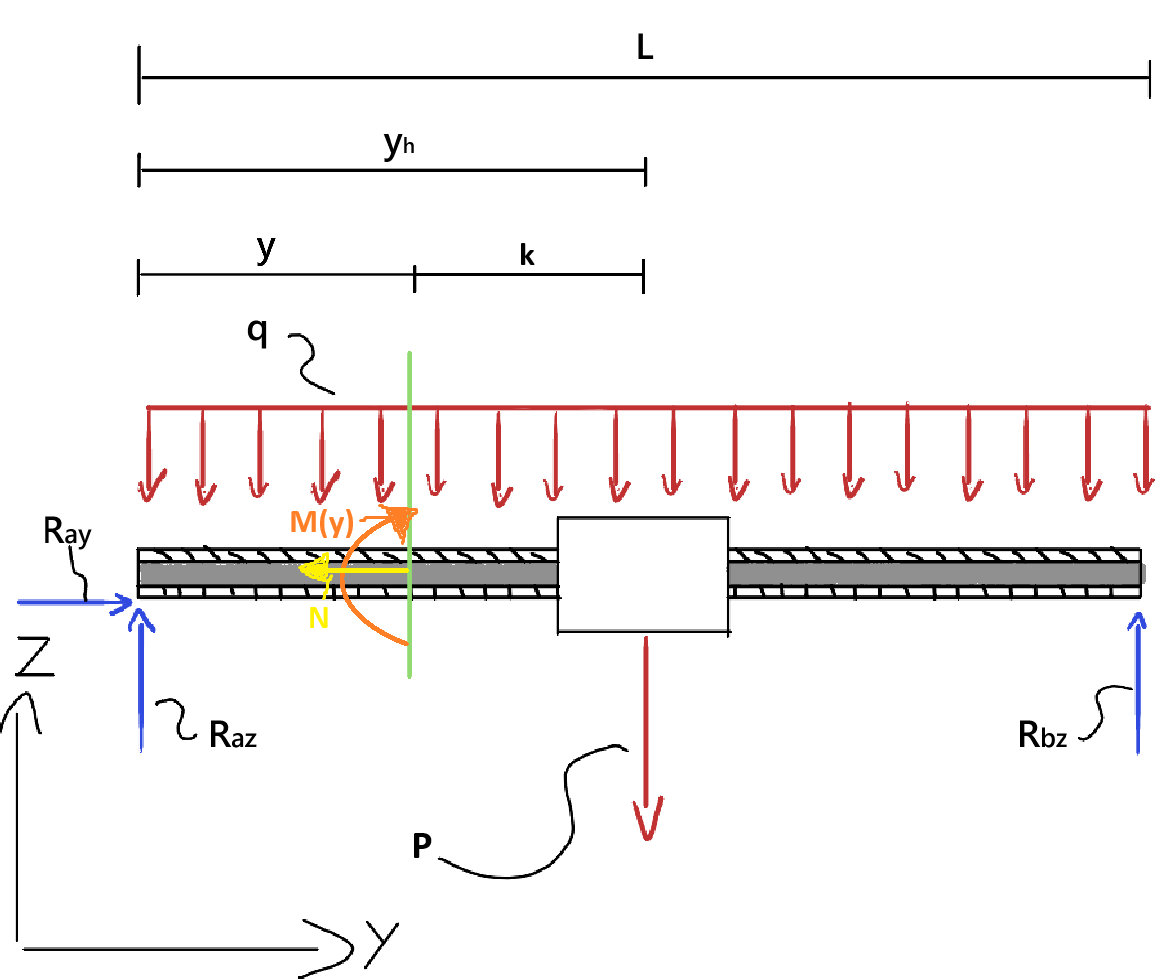
\includegraphics[width=0.5\linewidth]{Sections/6 Detaljeløsning/Media/FLD -snit.png}
    \caption{FLD af snit i stængerne på den lineære y-akse}
    \label{fig: Snit i y-akse}
\end{figure}

Her opstilles ligevægtsligningerne. Først formlen for normalkraften.
\begin{equation}\label{formel: snitnormal}
    N-R_{ay}=0
\end{equation}
Så findes momentet om snittet i tilfælde af, at P er placeret til højre for snittet.
\begin{equation} \label{formel: M_y_h>y(y)}
  \Sigma M_{y_h>y}(y)=0:\quad  M_{y_h>y}(y)- R_{az}\cdot y+\frac{q\cdot y^2}{2}=0
\end{equation}
Og igen i tilfælde af, at P er til venstre for snittet.
\begin{equation} \label{formel: M_y_h<y(y)}
   \Sigma M_{y_h<y}(y)=0:\quad  M_{y_h<y}(y)-R_{az}\cdot y+P\cdot(y-y_h)+\frac{q\cdot y^2}{2}=0
\end{equation}

Indsættes der værdier for reaktionskræfterne, og isoleres for snitkræfterne, vil formlerne for disse kræfter findes.
$R_{ay}$ kan omskrives fra formel \ref{formel: R_ay} og indsættes i formel \ref{formel: snitnormal}, og der kan isoleres for N, for at få et udtryk for normalkraften i stængerne.
\begin{equation}\label{formel: N=F}
    N=F
\end{equation}
$R_{bz}$ fra formel \ref{formel: R_bz} og $R_{az}$ fra formel \ref{formel: R_az} substitueres i \ref{formel: M_y_h>y(y)} og \ref{formel: M_y_h<y(y)}, hvorefter der isoleres for $M(y)$.
\begin{equation}\label{formel: M(y)1}
    M_{y_h<y}(y)= P\cdot y_h\cdot (1-\frac{ y}{L})+\frac {q\cdot( L \cdot y-y^2)}{2}
\end{equation}
\begin{equation} \label{formel: M(y)2}
   M_{y_h>y}(y)=P\cdot  (y-\frac{y_h\cdot y}{L})+ \frac {q\cdot( L \cdot y-y^2)}{2}
\end{equation}
Nu hvor de relevante snitreaktioner er fundet, kan normalspændingerne undersøges. Normalspændingerne fra træk/tryk kan beskrives ved formel \ref{formel: Kraft over areal}, der blev vist tidligere. Arealet i denne formel kommer fra to følgestænger som har et cirkulært tværsnit. Her kan arealet findes med formlen $A=\pi\cdot r^2$.\\
Kraften i denne formel kan findes igennem newtons anden lov der siger $F=m\cdot a$. Her er massen, massen af den vogn der kører langs akserne, den vil kaldes $m_v$. Accelerationen er den acceleration der kommer af vinkelaccelerationen motorerne skaber på skruerne. Accelerationen blev defineret i bilag \ref{Bilag - Bevægelse} til $a=\alpha \cdot O$, hvor $\alpha$ er vinkelaccelerationen og O er gevindhældningen i skruen. En formel for vinkelaccelerationen fra bilag \ref{Bilag - Bevægelse} kan erstatte $\alpha$. Til sidst, kan det tilføjes at vognen kan accelere i begge retninger, og kan derfor have begge fortegn. Formlen for kraften bliver derfor som det ses i formel \ref{formel: Accelerationskraft}.
\begin{equation} \label{formel: Accelerationskraft}
    F=\pm\frac{m_v\cdot \tau\cdot O}{m_l\cdot r_l^2}
\end{equation}
Nu er der et defineret udtryk kraften, som kan sættes ind i formel \ref{formel: Kraft over areal} samt formlen for arealet, for at finde spændingerne fra træk og tryk.
\begin{equation}\label{formel: Træk/tryk spændinger}
    \sigma_T=\pm\frac{m_v\cdot \tau\cdot O}{m_l\cdot r_l^2\cdot \pi \cdot r_f^2}
\end{equation}
I denne formel repræsenterer $m_v$ massen af vognen der bevæger sig, $\tau$ beskriver kraftmomentet i motoren, O beskriver som nævnt gevindhældningen, $m_l$ beskriver massen af ledeskruen, $r_l$ beskriver ledeskruens radius og $r_f$ beskriver følgestængernes radius.\\

Bøjningsspændinger fremgår af formel \ref{formel: momentspænding}. Det er interessant at finde de maksimale spændinger der kan gå igennem stangen, og derfor undersøges formel \ref{formel: M(y)1} og formel \ref{formel: M(y)2}, for det tilfælde med de største spændinger. Som nævnt tidligere er $y_h$ en uafhængig variabel der beskriver afstanden fra punkt a, hvor prikhovedet befinder sig. For at kunne vurdere prikhovedets placering og dets effekt på momentet, skrives $y_h$ om i de to formler. I formel \ref{formel: M(y)2} er prikhovedet til højre for snittet, derfor må det kunne skrives om til snittets placering plus en ekstra afstand altså $y_h=y+k$, hvor k er afstanden fra snittet til hovedets placering, som det ses på figur \ref{fig: Snit i y-akse}. Det samme kan skrives om i formel \ref{formel: M(y)1}, her er hovedet placeret til venstre for snittet, og der kan derfor trækkes en vilkårlig afstand fra snittes placering for at få hovedets placering. $y_h=y-k$ hvor k er afstanden fra hovedet til snittet.\\
Formel \ref{formel: M(y)2} skrives som nævnt over.
\begin{equation} \label{formel: M_y_h<y med k}
     M_{y_h<y}(y)= P\cdot (y-\frac{y^2}{L}+k\cdot (\frac{y}{L}-1))+\frac {q\cdot( L \cdot y-y^2)}{2}
\end{equation}
Det kan observeres i formel \ref{formel: M_y_h<y med k}, at $ y\cdot L^{-1} \leq 1$, fordi y ikke kan være større end L. Dette betyder, at k altid bliver ganget med et negativt tal i formel \ref{formel: M_y_h<y med k}. Derfor modarbejder et større k altid det samlede moments størrelse mere, som det er illustreret i figur \ref{fig: Afvigelse2}
Formel \ref{formel: M(y)1} skrives også om
\begin{equation} \label{formel: M_y_h>y med k}
   M_{y_h>y}(y)=P\cdot (y-\frac{y^2}{L}-k\cdot\frac{y}{L})+ \frac {q\cdot( L \cdot y-y^2)}{2}
\end{equation}
I denne formel tydeliggøres det, at hvis k vokser, sænkes det samlede moment i konstruktionen, da et negativt led vokser i størrelse med k. Dette ses også i figur 
\begin{figure}[H]
    \centering
    \begin{subfigure}[b]{0.48\textwidth}
           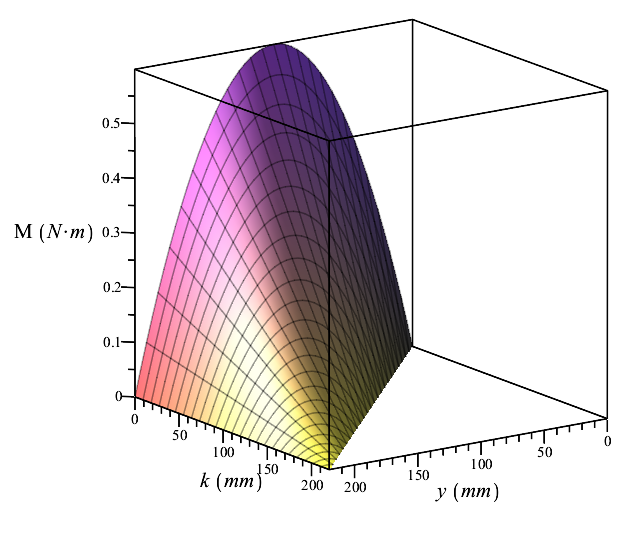
\includegraphics[width=\linewidth]{Sections/6 Detaljeløsning/Media/k2.png}
            \caption{3D-plot af moment med hensyn til snittes placering på stængerne, samt forskydning af last i forhold til snittets placering for ligning \ref{formel: M_y_h<y med k}}
            \label{fig: Afvigelse2}
    \end{subfigure}
    \begin{subfigure}[b]{0.48\textwidth}
           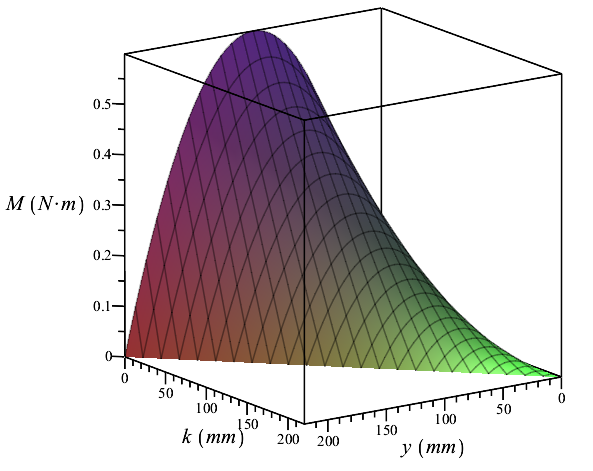
\includegraphics[width=\linewidth]{Sections/6 Detaljeløsning/Media/k1.png}
            \caption{3D-plot af moment med hensyn til snittes placering på stængerne, samt forskydning af last i forhold til snittets placering for ligning \ref{formel: M_y_h>y med k}}
            \label{fig: Afvigelse1}    
    \end{subfigure}
\end{figure}
        
Det konkluderes dermed, at de to formler har det største moment når punktlasten er placeret ovenpå snittet og k er 0, derfor kan formlen for det maksimale moment i alle punkter findes (\ref{formel: M_max(y)}), ved at sætte $k=0$ i \ref{formel: M_y_h>y med k} og \ref{formel: M_y_h<y med k}. De to formler bliver ens, og reduceres derfor til én.
\begin{equation} \label{formel: M_max(y)}
   M_{max}(y)= P\cdot (y-\frac{y^2}{L})+\frac {q\cdot( L \cdot y-y^2)}{2}
\end{equation}

Snitmomentet ${M_{max}(y)}$ kan herefter indsættes i formel \ref{formel: momentspænding} for momentspændingen.
\begin{equation} \label{formel: Momentspændninger med M_max}
    \sigma_M(y) =-\frac{P\cdot (y-\frac{y^2}{L})+\frac {q\cdot( L \cdot y-y^2)}{2}}{I}\cdot z
\end{equation}
I som er inertimomentet kan findes ved integrere højden fra neutralaksen i anden i forhold til arealet lagt til flytningsbidraget. Højden er i dette koordinatsystem z. Da de to følgestænger er placeret side om side, som det ses i figur \ref{fig: Flytningsbidrag2}, vil der ikke være nogen højdeforskel i arealtyngdepunktet imellem de to følgestænger, og derfor er flytningsbidraget i denne retning 0, og formlen bliver som formel \ref{formel: I_xx gennerelt}.
\begin{equation} \label{formel: I_xx gennerelt}
    I_{xx} = \int_{A} z^2 dA
\end{equation}
Som nævnt har følgestængerne et cirkulært tværsnit, dette afspejles i arealet. Her kan integralet omskrives til polære koordinater for nemmere at udregne integralet for det cirkulære tværsnit. Grænseværdierne bliver i cirklen en vinkel fra 0 til $2\pi$ og en radius fra 0 til r.
\begin{equation} \label{formel: I_xx cirkel udledning}
    I_{xx} =\int_0^{2\pi} \int_0^r r^3\cdot \sin(\theta) \ dr \ d\theta    
\end{equation}

Integrationen ender ud i udtrykket for formel \ref{formel: I_xx cirkel}
\begin{equation}\label{formel: I_xx cirkel}
    I_{xx} =\frac{\pi}{4}\cdot r^4  
\end{equation}

I dette tilfælde ganges $I_{xx}$ med to, fordi der er to følgestænger, for at give det totale inertimoment (\ref{formel: I_total}).
\begin{equation}\label{formel: I_total}
    I_{total} =2 \cdot I_{\textit{følgestænger}} = \frac{\pi}{2}\cdot r_f^4 
\end{equation}
Her er $r_f$ følgestængernes radius.

Dette indsættes i ligning \ref{formel: Momentspændninger med M_max}.
\begin{equation} \label{formel: momentspændning med M_max og I_total}
    \sigma_M(y) =-2\cdot\frac{P\cdot (y-\frac{y^2}{L})+\frac {q\cdot( L \cdot y-y^2)}{2}}{\pi\cdot r_f^4}\cdot z
\end{equation}

Det kan ses fra formlen ovenover, at spændingerne vokser med højdeforskellen i følgestængerne, derfor må de højeste spændinger findes i henholdsvist toppen og bunden følgestængerne. Z erstattes her med $\pm r_f$, som er følgestængernes radius, da det er den største højdeforskel, og vil give den største spænding. Momentets maksimum findes i midten af stængerne, altså ved $L/2$, og dette sættes ind for at finde de maksimale bøjningsspændinger.
\begin{equation}\label{formel: bøjningsspænding}
    \sigma_{M} =\pm\frac{(P+\frac {q\cdot L}{2})\cdot L}{2\cdot\pi\cdot r_f^3}
\end{equation}

Som nævnt tidligere findes træk og tryk spændingerne i samme plan som bøjningsspændingerne. Her gøres der derfor brug af superpositionsprincippet, og de to spændinger fra formel \ref{formel: Træk/tryk spændinger} og \ref{formel: bøjningsspænding} lægges sammen til at udlede den maksimale spændingsformel.
\begin{equation}\label{formel: Maksspænding}
    \sigma_{max}=\sigma_M+\sigma_T=\pm\frac{(P+\frac {q\cdot L}{2})\cdot L}{2\cdot\pi\cdot r_f^3}\pm\frac{m_v\cdot \tau\cdot O}{m_l\cdot r_l^2\cdot \pi \cdot r_f^2}
\end{equation}
Flydespændingen i stålet følgestængerne er lavet af, er $355$MPa. For at undersøge følgestængernes tykkelse, vil spændingen plottes i forhold til radius af følgestængerne. Dette ses på figur \ref{fig: Spænding i forhold til r}.
\begin{figure}[H]
    \centering
    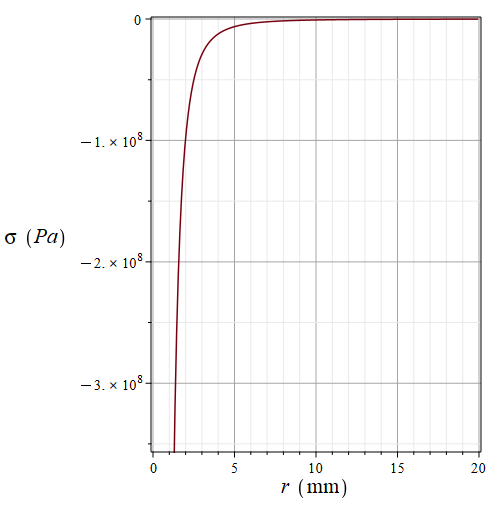
\includegraphics[width=0.55\linewidth]{Sections/6 Detaljeløsning/Media/Spænding ifht. r.png}
    \caption{Spændingsgraf i forhold til radius af følgestængerne}
    \label{fig: Spænding i forhold til r}
\end{figure}
På figuren ses det, at radius af følgestængerne skal være en smule større end $1$mm for at flydespændingerne ikke bliver opnået. På y-aksen skal radius være omkring $1$mm for ikke at overgå flydespændingen (Se bilag \ref{bilag- statik udledning}).

\begin{comment}
På grafen ses det som tidligere nævnt, at de største spændinger findes yderst i stangen. Derudover findes de ved det maksimale moment, i midten af stangen. Værdierne afhænger af radius af cylindrene, som det ses i formel \ref{Spændingsligning}, som der vil optimeres efter i senere afsnit.

    \[
\begin{Bsmallmatrix} \sigma_x \\ \sigma_y \\ \tau_{x,y} \end{Bsmallmatrix}
=
\begin{bsmallmatrix*}[r] \frac{(1-v)E}{(1+x(1-2v))} & \frac{v}{(1+x(1-2v))} & 0\\
    \frac{v}{(1+x(1-2v))} & \frac{(1-v)E}{(1+x(1-2v))} & 0 \\
    0 & 0 & G \end{bsmallmatrix*}
\begin{Bsmallmatrix} \epsilon_x \\ \epsilon_y \\ \epsilon_{x,y} \end{Bsmallmatrix}
\]
\end{comment}


\begin{figure}
    \centering
    \includegraphics[width=0.6\linewidth]{bilag/Media/Media/Spænding ifht. r1.png}
    \caption{Spænding i forhold til r på y-aksen}
    \label{fig: Spænding ifht. r1}
\end{figure}

\begin{figure}
    \centering
    \includegraphics[width=0.6\linewidth]{bilag/Media/Media/Udbøjning ifht. r1.png}
    \caption{Udbøjning i forhold til r på y-aksen}
    \label{fig: Udbøjning ifht. r1}
\end{figure}

